\documentclass[tikz,border=5pt]{standalone}
\usepackage[T1]{fontenc}
\usepackage{lmodern,amsmath,amssymb}
\usetikzlibrary{arrows.meta,calc,positioning,fit,backgrounds,shapes.geometric,matrix,decorations.pathreplacing,patterns}
\definecolor{ink}{gray}{0.08}
\definecolor{wash}{gray}{0.965}
\definecolor{soft}{gray}{0.45}
\tikzset{box/.style={draw=ink,line width=.65pt,fill=white,align=center,inner sep=4pt,outer sep=0pt,font=\small},flow/.style={draw=ink,line width=.65pt,-{Latex[length=1.8mm,width=1.3mm]},rounded corners=2pt},annotation/.style={font=\scriptsize,text=soft,align=center},groupbox/.style={draw=soft,dashed,line width=.45pt,fill=wash}}
\begin{document}
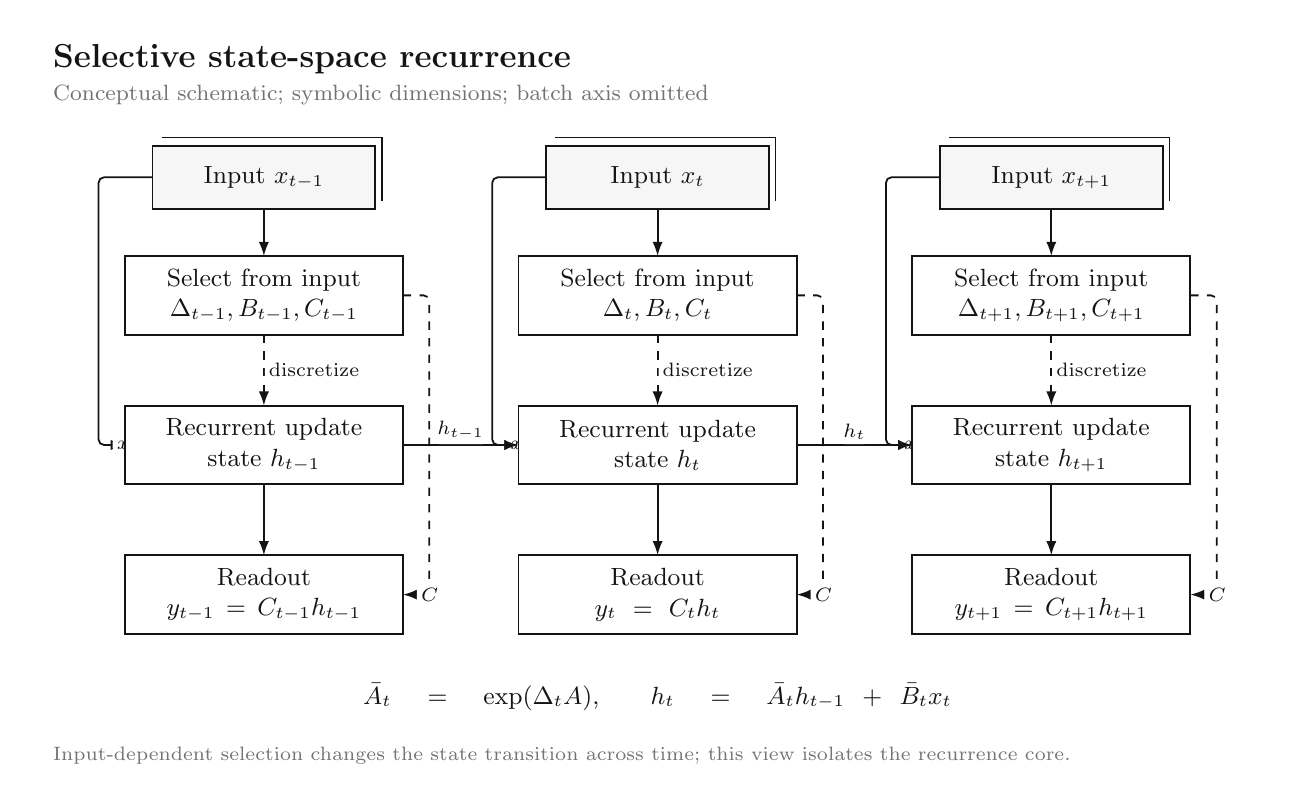
\begin{tikzpicture}[x=1cm,y=-1cm,font=\rmfamily,text=ink]

\path[use as bounding box] (0,0) rectangle (16,9.5);
\node[anchor=west,font=\large\bfseries] at (.2,.4) {Selective state-space recurrence};
\node[anchor=west,font=\footnotesize,text=soft] at (.2,.85) {Conceptual schematic; symbolic dimensions; batch axis omitted};
\begin{pgfonlayer}{background}
\end{pgfonlayer}
\node[box,fill=wash,minimum width=2.8cm,minimum height=0.8cm,text width=2.55cm] (xa) at (3,1.9) {Input $x_{t-1}$};
\draw[ink,line width=.4pt] (1.7000000000000002,1.4) -- (4.5,1.4) -- (4.5,2.1999999999999997);
\node[box,minimum width=3.5cm,minimum height=1.0cm,text width=3.25cm] (sela) at (3,3.4) {Select from input\\$\Delta_{t-1},B_{t-1},C_{t-1}$};
\node[box,minimum width=3.5cm,minimum height=1.0cm,text width=3.25cm] (ha) at (3,5.3) {Recurrent update\\state $h_{t-1}$};
\node[box,minimum width=3.5cm,minimum height=1.0cm,text width=3.25cm] (ya) at (3,7.2) {Readout\\$y_{t-1}=C_{t-1}h_{t-1}$};
\node[box,fill=wash,minimum width=2.8cm,minimum height=0.8cm,text width=2.55cm] (xb) at (8,1.9) {Input $x_{t}$};
\draw[ink,line width=.4pt] (6.699999999999999,1.4) -- (9.5,1.4) -- (9.5,2.1999999999999997);
\node[box,minimum width=3.5cm,minimum height=1.0cm,text width=3.25cm] (selb) at (8,3.4) {Select from input\\$\Delta_{t},B_{t},C_{t}$};
\node[box,minimum width=3.5cm,minimum height=1.0cm,text width=3.25cm] (hb) at (8,5.3) {Recurrent update\\state $h_{t}$};
\node[box,minimum width=3.5cm,minimum height=1.0cm,text width=3.25cm] (yb) at (8,7.2) {Readout\\$y_{t}=C_{t}h_{t}$};
\node[box,fill=wash,minimum width=2.8cm,minimum height=0.8cm,text width=2.55cm] (xc) at (13,1.9) {Input $x_{t+1}$};
\draw[ink,line width=.4pt] (11.7,1.4) -- (14.5,1.4) -- (14.5,2.1999999999999997);
\node[box,minimum width=3.5cm,minimum height=1.0cm,text width=3.25cm] (selc) at (13,3.4) {Select from input\\$\Delta_{t+1},B_{t+1},C_{t+1}$};
\node[box,minimum width=3.5cm,minimum height=1.0cm,text width=3.25cm] (hc) at (13,5.3) {Recurrent update\\state $h_{t+1}$};
\node[box,minimum width=3.5cm,minimum height=1.0cm,text width=3.25cm] (yc) at (13,7.2) {Readout\\$y_{t+1}=C_{t+1}h_{t+1}$};
\node[align=center,inner sep=0pt,outer sep=0pt,font=\small,minimum width=13cm,minimum height=0.6cm,text width=12.75cm] (note12) at (8,8.5) {$\bar A_t=\exp(\Delta_t A)$,\qquad $h_t=\bar A_t h_{t-1}+\bar B_t x_t$};
\begin{pgfonlayer}{background}
\draw[flow] (xa.south) -- (sela.north);
\draw[flow] (xa.west) -- (0.8999999999999999,1.9) -- (0.8999999999999999,5.3) -- (ha.west) node[midway,right,fill=white,inner sep=1.5pt,font=\scriptsize] {$x$};
\draw[flow,dashed] (sela.south) -- (ha.north) node[midway,right,fill=white,inner sep=1.5pt,font=\scriptsize] {discretize};
\draw[flow] (ha.south) -- (ya.north);
\draw[flow,dashed] (sela.east) -- (5.1,3.4) -- (5.1,7.2) -- (ya.east) node[midway,right,fill=white,inner sep=1.5pt,font=\scriptsize] {$C$};
\draw[flow] (xb.south) -- (selb.north);
\draw[flow] (xb.west) -- (5.9,1.9) -- (5.9,5.3) -- (hb.west) node[midway,right,fill=white,inner sep=1.5pt,font=\scriptsize] {$x$};
\draw[flow,dashed] (selb.south) -- (hb.north) node[midway,right,fill=white,inner sep=1.5pt,font=\scriptsize] {discretize};
\draw[flow] (hb.south) -- (yb.north);
\draw[flow,dashed] (selb.east) -- (10.1,3.4) -- (10.1,7.2) -- (yb.east) node[midway,right,fill=white,inner sep=1.5pt,font=\scriptsize] {$C$};
\draw[flow] (xc.south) -- (selc.north);
\draw[flow] (xc.west) -- (10.9,1.9) -- (10.9,5.3) -- (hc.west) node[midway,right,fill=white,inner sep=1.5pt,font=\scriptsize] {$x$};
\draw[flow,dashed] (selc.south) -- (hc.north) node[midway,right,fill=white,inner sep=1.5pt,font=\scriptsize] {discretize};
\draw[flow] (hc.south) -- (yc.north);
\draw[flow,dashed] (selc.east) -- (15.1,3.4) -- (15.1,7.2) -- (yc.east) node[midway,right,fill=white,inner sep=1.5pt,font=\scriptsize] {$C$};
\draw[flow] (ha.east) -- (hb.west) node[midway,above,fill=white,inner sep=1.5pt,font=\scriptsize] {$h_{t-1}$};
\draw[flow] (hb.east) -- (hc.west) node[midway,above,fill=white,inner sep=1.5pt,font=\scriptsize] {$h_t$};
\end{pgfonlayer}
\node[anchor=west,align=left,font=\scriptsize,text=soft,text width=15.6cm] at (.2,9.25) {Input-dependent selection changes the state transition across time; this view isolates the recurrence core.};
\end{tikzpicture}
\end{document}
